% !TEX root = ../main.tex
\lecture{6}{2026-10-21}{Marketing Intro Lernvideos/Vorlesung}

\section{Marketing}

\begin{definition}
    [Marketing] besteht aus Handlungen, die Austauschbeziehungen zwischen Parteien ermöglichen und aufrechterhalten.
\end{definition}

\subsection{Ziel}
Ziel des Markting ist: wichtige Bedürfnisse einer erreichbaren und monetär attraktiven Zielgruppe durch massgeschneiderte Produktangebote mit besserem Nutzen/Kosten verhältnis als die Konkurrenz dauerhaft und nachhaltig bedienen.\footnote{Die aktive Rolle von marketing in der Erzeugung von Wünsche und Einfluss auf Konsumentenverhaltens nicht erwähnt}

\subsection{Effekte erfolgreiches Marketing}

\begin{itemize}
    \item Steigerung des Produktnutzens für Konsumenten
    \item Reduktion der \textit{Floprate}/sinnlose produkte
    \item Sogsamer Umgang mit Ressourcen
    \item Reduzierte Suchzeit für Kunden
\end{itemize}

\subsection{Der Marketingprozess und Begriffe}
Marketing kann als Prozess verstanden werden

\subsubsection{Begriffe}

\begin{itemize}
    \item Bedürfnis: Zustand von empfundener Mangel
    \item Wünsche, Form des Bedürfnisses nach kultur, soziales Milieu, individuell (bei durst tee, wasser, saft)
    \item Nachfrage: Kunden mit wünsche und genugend Kaufkraft \footnote{Diejenigen mit denselben Bedürfnissen ohne die sozialen Mittel sich diese anzueignen werden nicht bedient}
    \item Produkte: Angebote auf Markt zur Befriedigung von Wünschen und Bedürfnisse
\end{itemize}

\subsubsection{Schritte und Teilaufgaben}

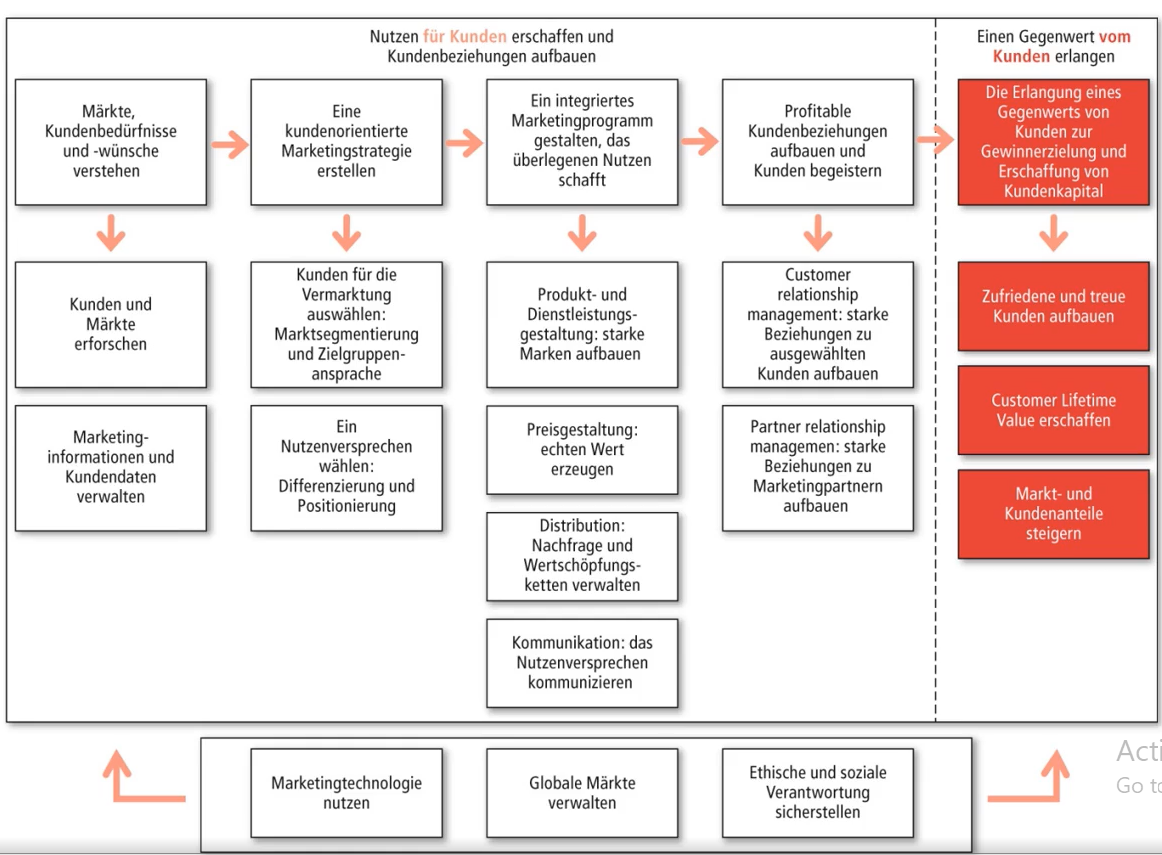
\includegraphics[width=\textwidth,height=0.7\textheight,keepaspectratio]{figures/Marktingschritte.png}


\subsubsection{Kunden kaufen nicht Produkte}

\begin{itemize}
    \item sondern nach Nutzen abhängig von wahrnehmung der Leistung des Produkts und Erwartungen
    \item Entscheidungen nach wahrgenommenen Kosten negative nutzen
    \item wahrgenommenen konvergente Nutzen deuten auf Konkurrenz hin
    \item divergente Nutzen oder differenzierung dienen der Verbesserung vom Kundenverständnis
\end{itemize}

\subsubsection{Arten von Märktetrennung}

\begin{itemize}
    \item Produktmarkt
    \begin{itemize}
        \item Sektoren nach spezifischen Produkten geteilt (Früchte, Autos, Uhren etc)
    \end{itemize}
    \item Bedarfsmarktkonzept 
    \begin{itemize}
        \item Nach Bedürfnis oder Wünsche (Essen, Transport, Status)
    \end{itemize}
\end{itemize}
\pagebreak
\subsection{Marktforschung MaFo}

\subsubsection{4 Stufen}

\begin{enumerate}
    \item Problemdefinition und Zielsetzung 
    \item Unterschungsplan
    \item Datenerhebung 
    \item Interpretation und Kommunikation der Ergebnisse
\end{enumerate}

\subsubsection{3 Arten von Forschungszielen}

\begin{itemize}
    \item Explorativ => Bei neuer Markt(neue Bedürnisse/Wünsche oder Produkt) oder fehlende Vorinformationen
    \item Deskriptiv => umfassende Beschreibung, Marktpotenzial, Demografie etc.
    \item Explikativ => Kausalitäten aufdecken
\end{itemize}

\subsubsection{Untersuchungsmethoden}
\begin{itemize}
    \item Befragung: Interviews zur Erhebung primärer Daten
    \item Beobachtungen: aus bestehenden Daten oder passive Datenerhebung
    \item Experimente:
    \begin{itemize}
        \item Labor (Simulationen)
        \item Feld
    \end{itemize}
\end{itemize}

\subsubsection{Datenerhebung}

\begin{definition}
    [Stichprobe] ist die Datenerhebung auf einer Teilmenge der Zielgruppe, die repräsentativ aus Verhältnismässig gleiche Merkmalen besteht
\end{definition}

\textbf{Entscheidungen}
\begin{itemize}
    \item Welche Subjekte
    \item Grösse
    \item Verfahren
\end{itemize}

\textbf{Bewertungskriterien}
\begin{itemize}
    \item Objektivität
    \item Reliabilität (Genauigkeit, Reproduzierbarkeit)
    \item Validität (relevante Merkmale wurden gemessen)
\end{itemize}

\textbf{Verfahren} \break
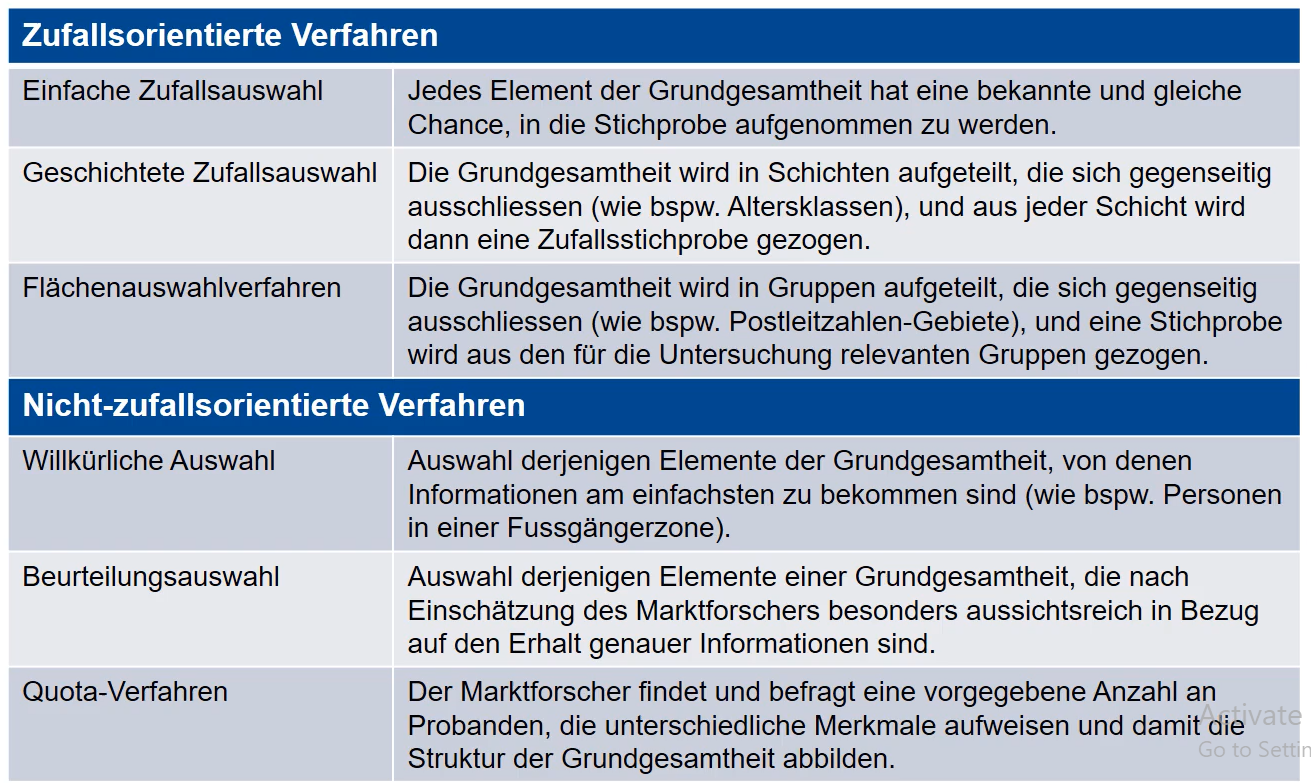
\includegraphics[width=\textwidth,height=0.7\textheight,keepaspectratio]{figures/Marketingverfahren.png}


\subsection{Konsumentenverhalten}


\subsubsection{Entscheidungsschritte}

\begin{enumerate}
    \item Wahrnehmung
    \item Suche und ihre Intensität bestimmt durch:
    \begin{itemize}
        \item Unterschiede der Produktmerkmale der Konkurrenten
        \item Involvement (wie wichtig das gesuchte Produkt für den Konsument ist)
        \item 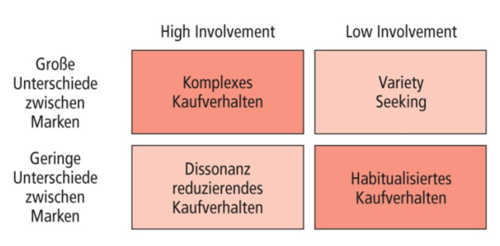
\includegraphics[width=\textwidth,height=0.7\textheight,keepaspectratio]{figures/Kaufverhalten.png}
    \end{itemize}
    \item Bewertung Alternativen
    \item Kaufentscheidung
    \item Nachkaufphase
\end{enumerate}

\pagebreak
\subsubsection{SOR-Modell}

\begin{definition}
    [Stimulus-Organism-Response] Modell zur darstellung der Phasen des internen Entscheidungsprozesses. Über Anreize, die vom Organismus (als BlackBox betrachtet) interpretiert werden, werden Handlungen/Entscheidungen getroffen.
\end{definition}

\subsubsection{Persönliche Faktoren}

\begin{itemize}
    \item Persönlichkeit
    \begin{itemize}
        \item Einzigartige psychische Merkmale, die zur relativ stabilen und vorhersehbaren Reaktionen auf Umfeld führen.
    \end{itemize}
    \item Selbstbild 
    \begin{itemize}
        \item Wahrnehmung der Person von sich selbst.
    \end{itemize}
\end{itemize}

\subsection{B2C Beziehung}

\begin{definition}
    [B2C] Business-To-Customer. Unternehmen verkauf direkt an Endkonsumenten des Produkts
\end{definition}

\subsubsection{Dual Entitlement}
Unterschiedlich zu B2B Beziehungen, worin Unternehmen untereinander handeln, ist in B2C-Beziehungen die Subjektivität der Kunden einflussreicher auf die Kaufentscheidung und Kaufgewohnheiten.
\begin{definition}
[Dual-Entitlement] beschreibt die Erwartungen der Parteien (Business und Customer),die sich auf Referenzwerte basieren, in Bezug auf eventuelle Preisveränderungen eines Produkts.
    
\end{definition}

\begin{itemize}
    \item Kunden vergleichen aktuellen Preis mit der Referenztransaktion des letztes Kaufes.
    \item Anbieter vergleichen es mit Referenzgewinne und geben Kostenweiter um diesen beizubehalten
    \item Kostenweitergabe wird als fair betrachtet (z.B. erhöhte Produktionskosten), während Ausnutzen von Knappheit für Preiserhöhung zum gleichen Betrag als unfair empfunden wird 
    \item \textbf{Take-away} Konsumenten, die weiterhin ausreichende Kaufkraft besitzen, sind bereit Preiserhöhungen zu akzeptieren bei vernunftigen Begründungen 
\end{itemize}
\pagebreak
Um die Dauerhaftigkeit der Kundenbeziehungen und Verkaufschancen zu sichern, sollte man in einer Situation von Knappheit versuchen nicht rein über erhöhte Preise Gewinne zu erzielen, sondern über andere Methoden:
\begin{itemize}
    \item Allokation (Gewisse Konsumentengruppen oder Produktvarianten nicht mehr produkzieren)
    \item Offene Kommunikation (Begründung der Preiserhöhungen)
    \item Gleichbleibende Preise, aber reduzierte qualität (USB sticks mit etwas weniger Speicherplatz, solang noch nützlich für die Kunden)
    \item Kosten teilweise selbst tragen
\end{itemize}

\subsection{Marktreaktionen: Folgen von maximaler Preismacht}

\begin{enumerate}
    \item Weitergabe an Endkonsumenten      
    \item Nachfrage reduziert (Wohlfahrtsverlust)
    \item Kunden sichern sich langfristig ab (langfristige, geregelte verträge)
    \item Neue Wettbewerber (Hohe Gewinne sind attraktiv, und möglichkeit Markanteil gewinnen, wenn günstigerer Preis angeboten werden kann)
    \item Entscheidungen der Anbieter über Allokation (Streichung von Produktsegement, Priorisierung von Lieferanten etc.)  
\end{enumerate}

\subsection{Marktforschung und Luxusmarken}

\subsubsection{Signaling theorie}
\begin{itemize}
    \item Die Begierde nach einem Luxusprodukt ist abhängig von:
    \begin{itemize}
        \item steigt direkt mit der Bekanntheit 
        \item und negativ zur Verbreitung 
    \end{itemize}
\end{itemize}

\textbf{Merksatz}: Bekanntheit macht Signal lesbar für andere, Seltenheit gibt Status/aussagekräftigkeit
\pagebreak
\subsubsection{Untersuchungsverfahren}
Auf Basis der Signaling theorie wurde die Frage der Festlegung eines Angebotslimits bei Luxusmarken untersucht. 
Sie wählten die Zufällige Stichprobe als passendste Methode zur Datenerhebung, da das Ziel war einerseits zu messen, welche Marken am meisten gewünscht sind,
und anderseits die Bekanntheit der Marken zu messen nicht nur über die Konsumenten die es bereits kennen (in der Bubble sind), sondern in der allgemeinen Bevölkerung.